% ---
% Capitulo de revisão de literatura
% ---


\chapter{Trabalhos Relacionados}\label{referencial_teorico}
Aqui será dedicado a descrever os trabalhos relacionados, descrevendo cada um dos estudos 
e abordando seus pontos fortes e fracos. O autor \cite{Garcia} define uma serie de estrategias 
para avaliar um RTOS moderno, passando por diversos pontos importantes em um sistema de tempo real, 
como resposta a eventos externos, compartilhamento de recurso e sincronização entre tarefas. 
Em \cite{Raymundo} o autor se baseia nestas estrategias, 
implementando com novas tecnicas em 5 sistemas operacionais diferentes, inclusive nos dois 
sistemas propostos aqui neste trabalho, seu trabalho tem um foque em internet das coisas, 
tendo como base a plataforma de hardware NXP/Freescale FRDM-K64F.
No estudo \cite{nicolas2019avaliaccao}, o autor busca compreender e avaliar o funcionamento 
do FreeRTOS embarcado em um cubesat real, o estudo explica o funcionamento do sistema em 
cada um de seus pontos como, controle e escalonamento de tarefas, gerenciamento de filas e 
meemória, erros comuns e etc. Para avaliar o sistema, o mesmo foca numa serie de experimentos 
que são voltados ao funcionamento do sistema em um ambiente real de operação, tendo como vista 
problemas relacionados a radiação, perca de memória, corrompimento de dados e estouro de memória.
Os trabalhos trabalhos de \cite{Garcia} e \cite{Raymundo} tem foque nas qualidades do sistema, já 
o trabalho de \cite{nicolas2019avaliaccao} foca no desenpelho do sistema em ambiente real, perante 
a problemas externos e de missão.

\chapter{Revisão Bibliométrica sobre CubeSats e Zephyr RTOS}\label{referencial_teorico}

Nesta seção são consideradas informações referentes á produção acadêmica mundial, que 
abordam os temas Zephyr RTOS, CubeSats e Sistemas Operacionais de tempo real aplicados 
em plataformas de Nano-Satélites e CubeSats, foi realizada uma revisão bibliométrica 
sobre estes temas. 


Com a miniaturização e industrialização de componentes eletrônicos antes inacessíveis 
público comum, permitiu-se que diversas missões espaciais pudessem ser elaboradas rapidamente 
e com um baixo custo de produção, levando ao desenvolvimento de satélites menores que passaram 
não somente de ferramentas educacionais, mas para uma plataforma padrão de tecnologia e 
instrumentação científica \cite{Selva2012}. Estas plataformas construídas com componentes de 
prateleira (COTS) desenvolvidas em forma de cubo, possibilitam pesquisas científicas já cada 
vez mais reconhecidas com recursos de instrumentação que foram aplicadas em satélites maiores, 
promovendo a pesquisa em ambiente espacial antes restrito a grande agentes, agora a 
universidades e países em desenvolvimento \cite{Woellert2011}.


A Figura~\ref{fig: CubeSat NanoSatC-Br2} mostra o um dos CubeSats desenvolvido no Brasil pela Universidade 
Federal de Santa Maria (UFSM) com apoio da Agência Espacial Brasileira (AEB), Ministério de Ciência e 
Tecnologia (MCTI) e do Instituto Nacional de Pesquisas Espaciais (INPE).

\begin{figure}[H]
	\centering
	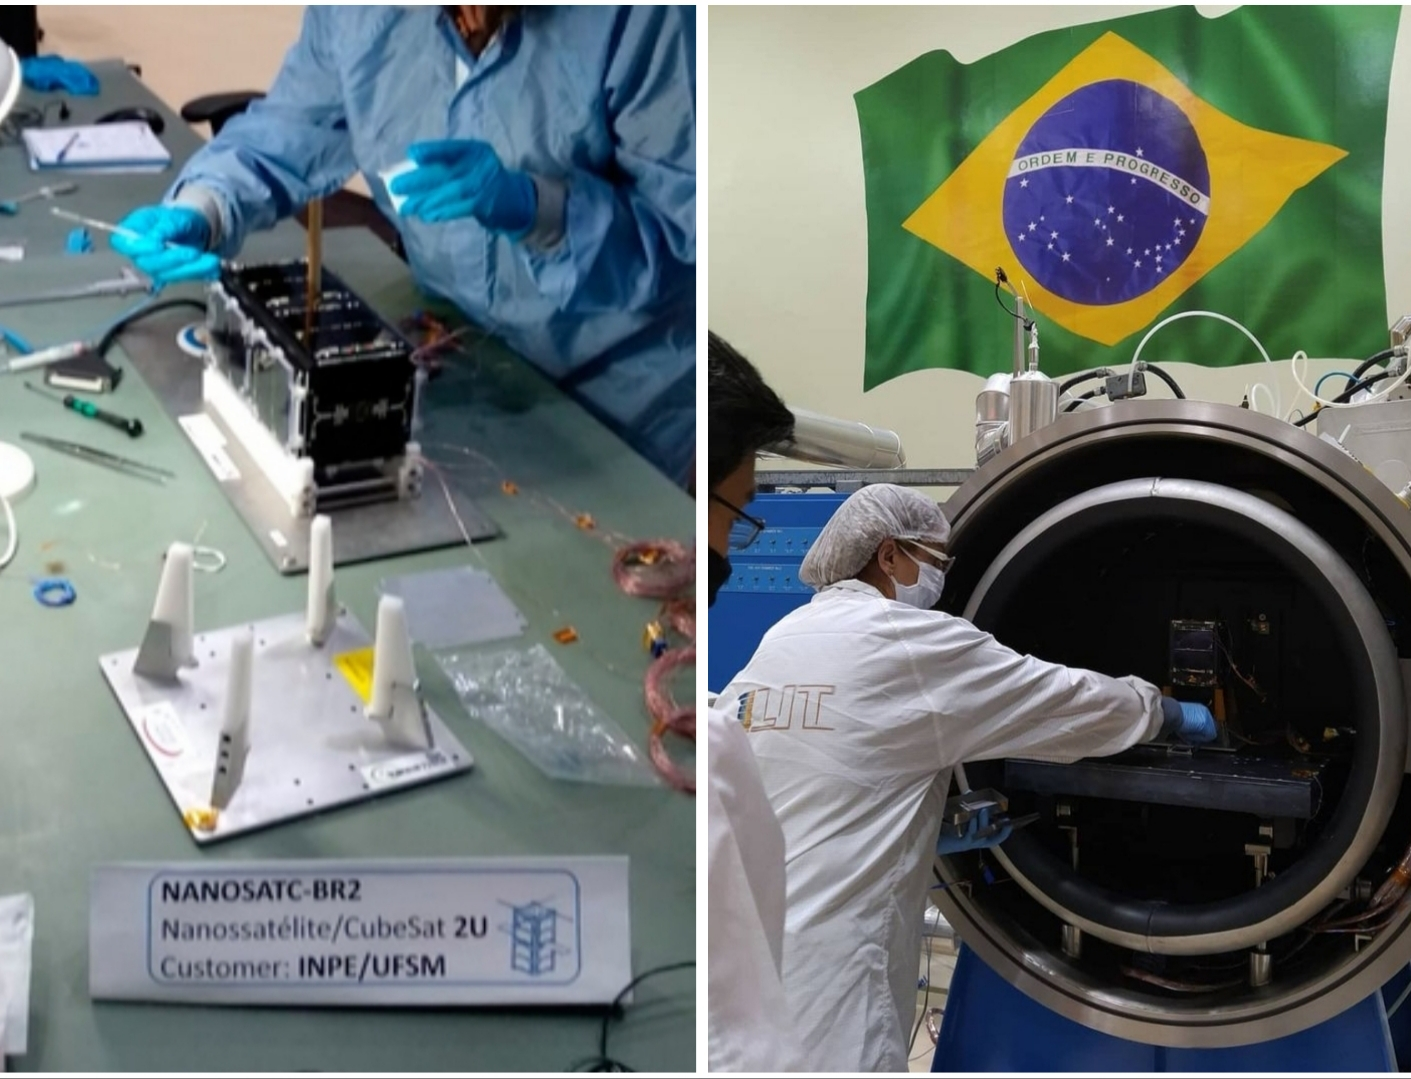
\includegraphics[width=15cm]{imagens/cubesat_brasil.jpg}
	\caption{NanoSatC-Br2 durante o processo de integração e teste no LIT/INPE}
	Fonte: Portal "www.tecnoveste.com.br", Lançamento de mais um satélite brasileiro – NanoSatC-Br2.
	\label{fig: CubeSat NanoSatC-Br2}
\end{figure}

\subsection{Zephyr RTOS}
Há mais de 20 anos nascia o primeiro RTOS do mercado, desde então outros sistemas tem trazido 
contribuições para o mundo embarcado. Um sistema operacional de tempo real se difere de um sistema 
operacional comum por depender diretamente do momento em que a ação foi produzida, buscando 
manter o tempo de mudança de contexto mínimo e gerenciando a execução de tarefas de acordo com 
suas prioridades \cite{Hambarde}. Os aplicativos de tempo real se tornaram populares devido a 
complexidade dos sistemas modernos, paralelo a isso o mercado de RTOS é bastante grande, com 
diversos antagonistas fornecendo ferramentas para resolver problemas de tempo real em diversas 
plataformas e de diversas maneiras, tornando a escolha cada vez mais difícil \cite{Hambarde}.


Zephyr é um RTOS de código aberto gerido pela Linux Foundation, construído sobre recursos
limitados e pensado em segurança e proteção, frequentemente adotado em sistemas críticos \cite{Zhao}.
Suportando uma grande variedade de placas de hardware e utilizado por empresas como Google, Intel
e Facebook. Oferece cooperatividade e segmentação preemptiva, alocação estática de memória,
isolamento de thread e dispositivos de proteção de memória \cite{nyffenegger2020connecting}.

\begin{figure}[H]
	\centering
	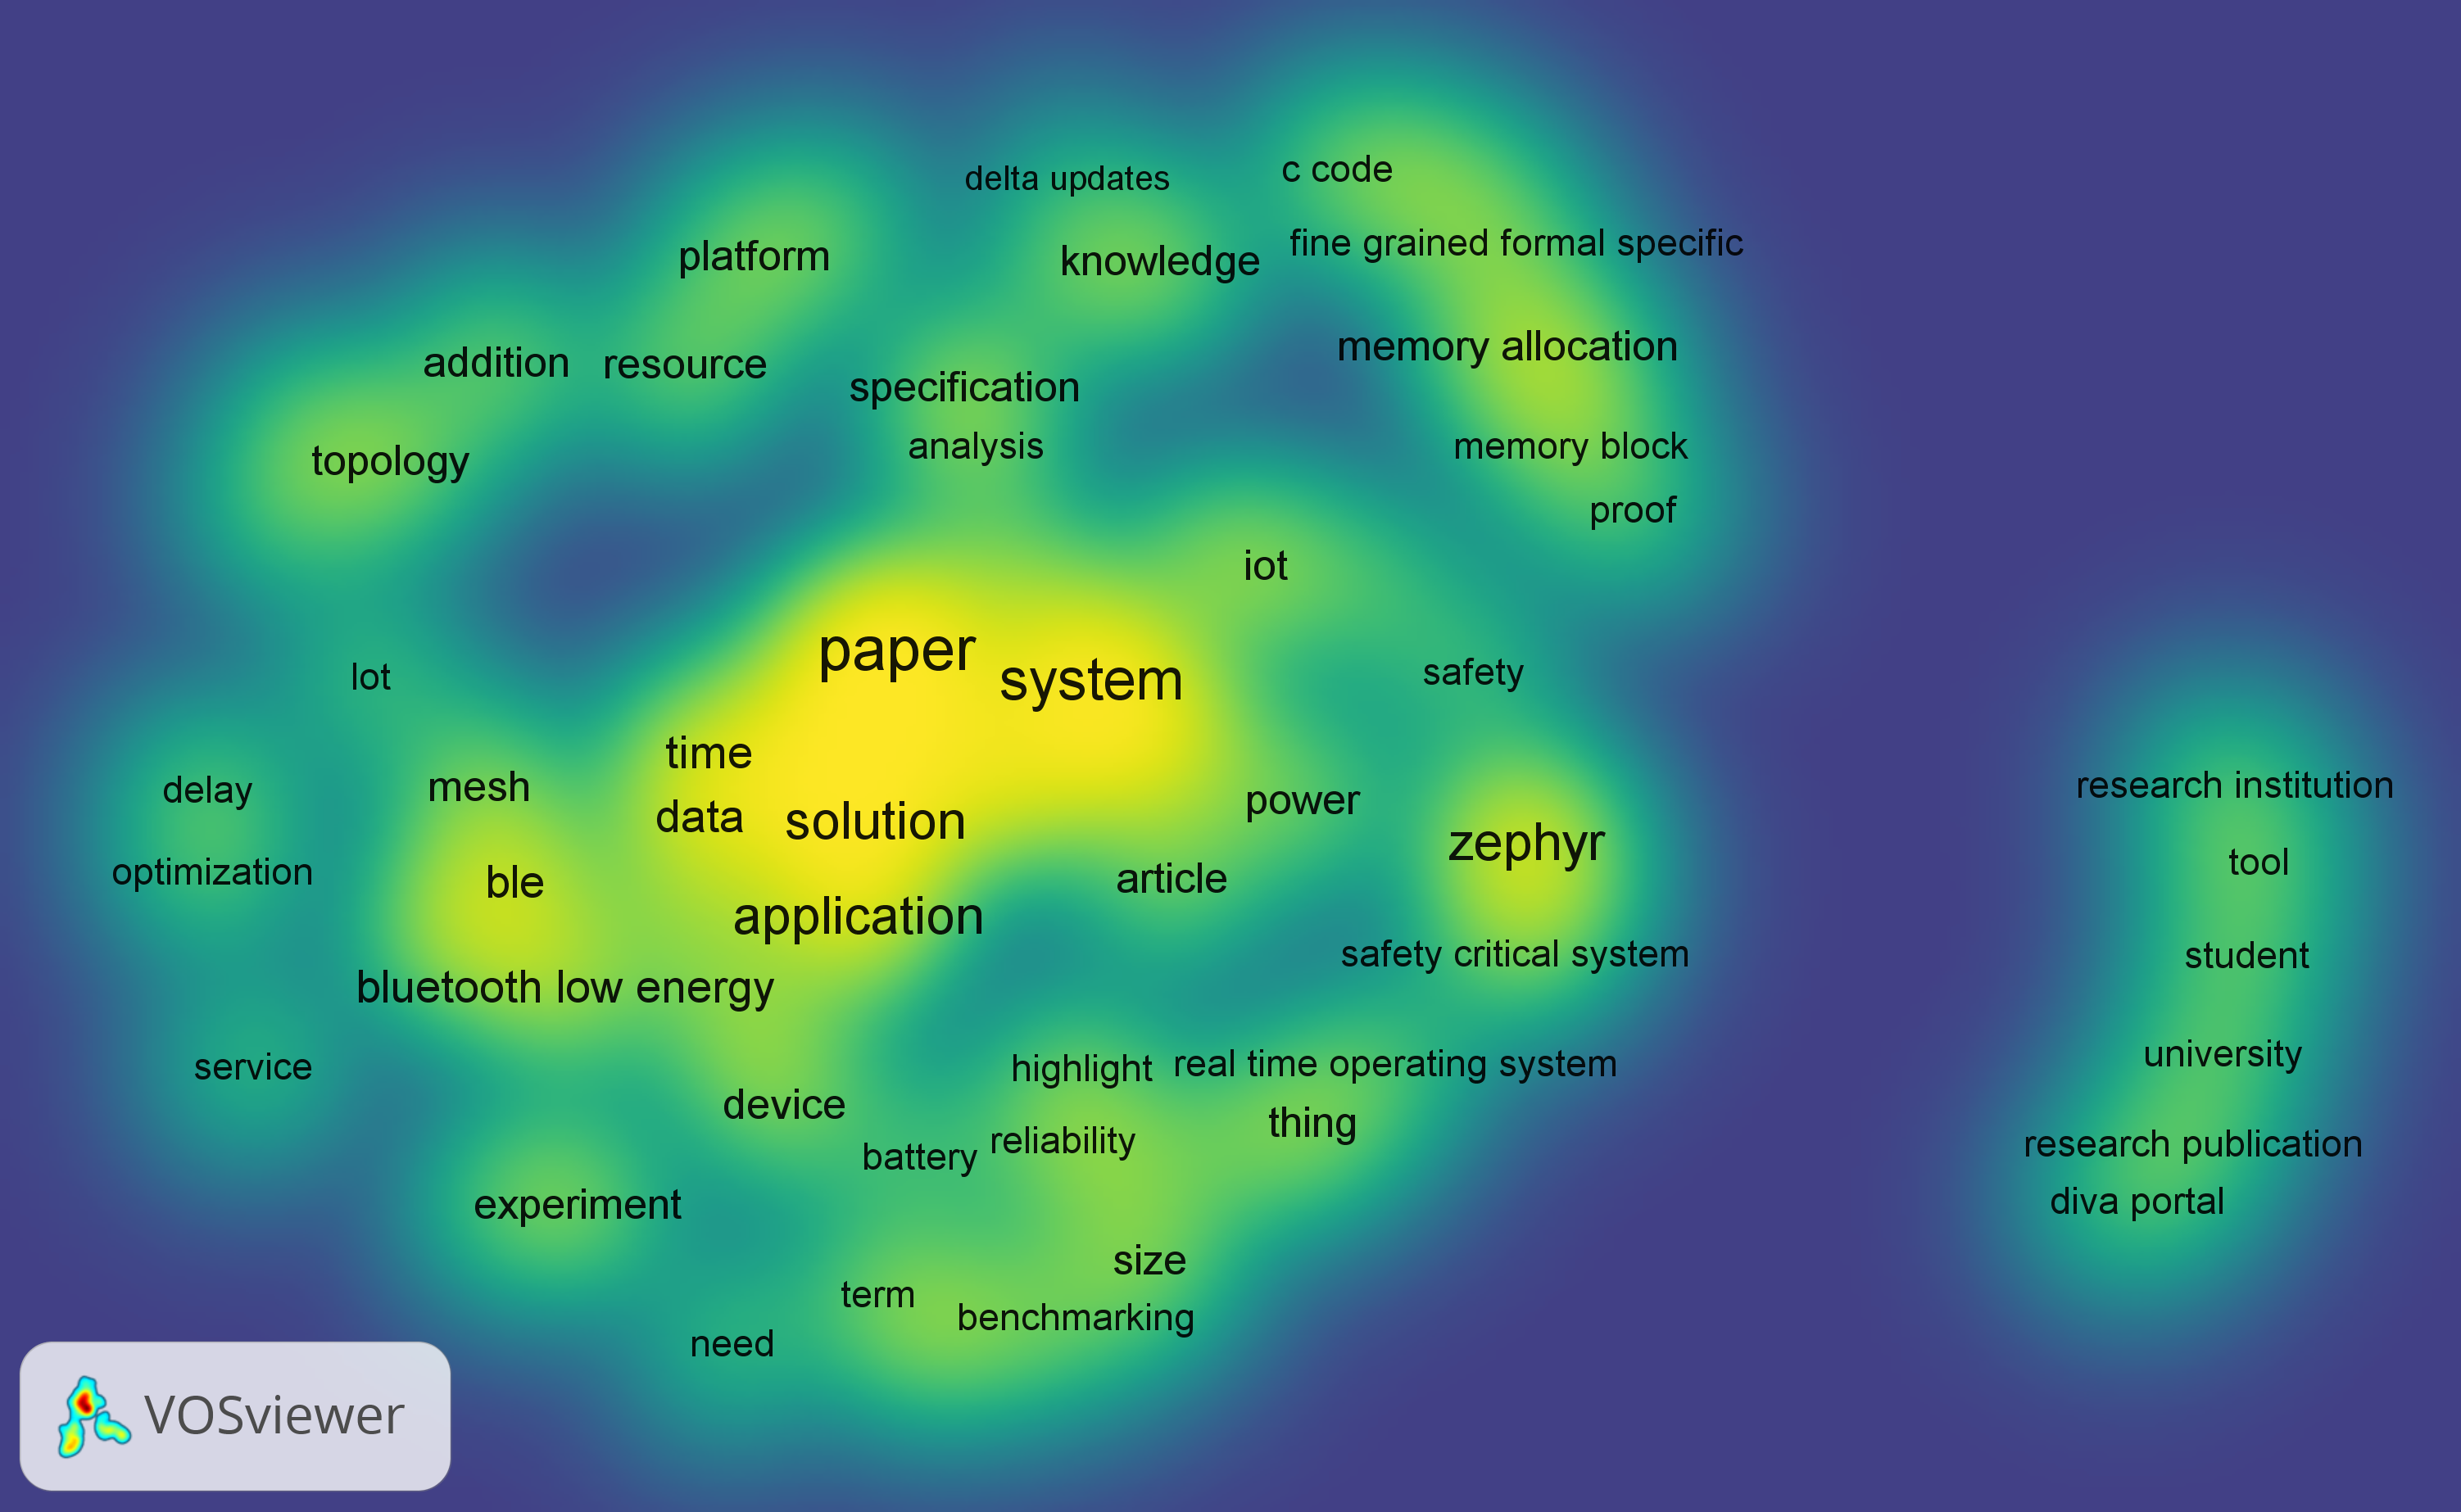
\includegraphics[width=15cm]{imagens/Zephyr_RTOS_Density_Visualization.png}
	\caption{Mapa de visualização de densidade sobre o termo "Zephyr RTOS"}
	Fonte: Autor com base no Software VOSViwer.
	\label{fig: Zephyr Density Visualization}
\end{figure}

A Figura~\ref{fig: Zephyr Density Visualization} representa uma espécie de "mapa de calor" sobre o 
tema "Zephyr RTOS" no mecanismo de busca Google Scholar, ao seu redor pode-se notar termos que 
remetem a RTOS como "safety critical system", "iot", "bluetooth low energy" e "memory allocation". 
Também e possível notar os termos "solution", "application", "service" e "plataform" que reforçam a 
ideia de que zephyr é amplamente utilizada em diversas plataformas e projetos\cite{nyffenegger2020connecting}.

\begin{figure}[H]
	\centering
	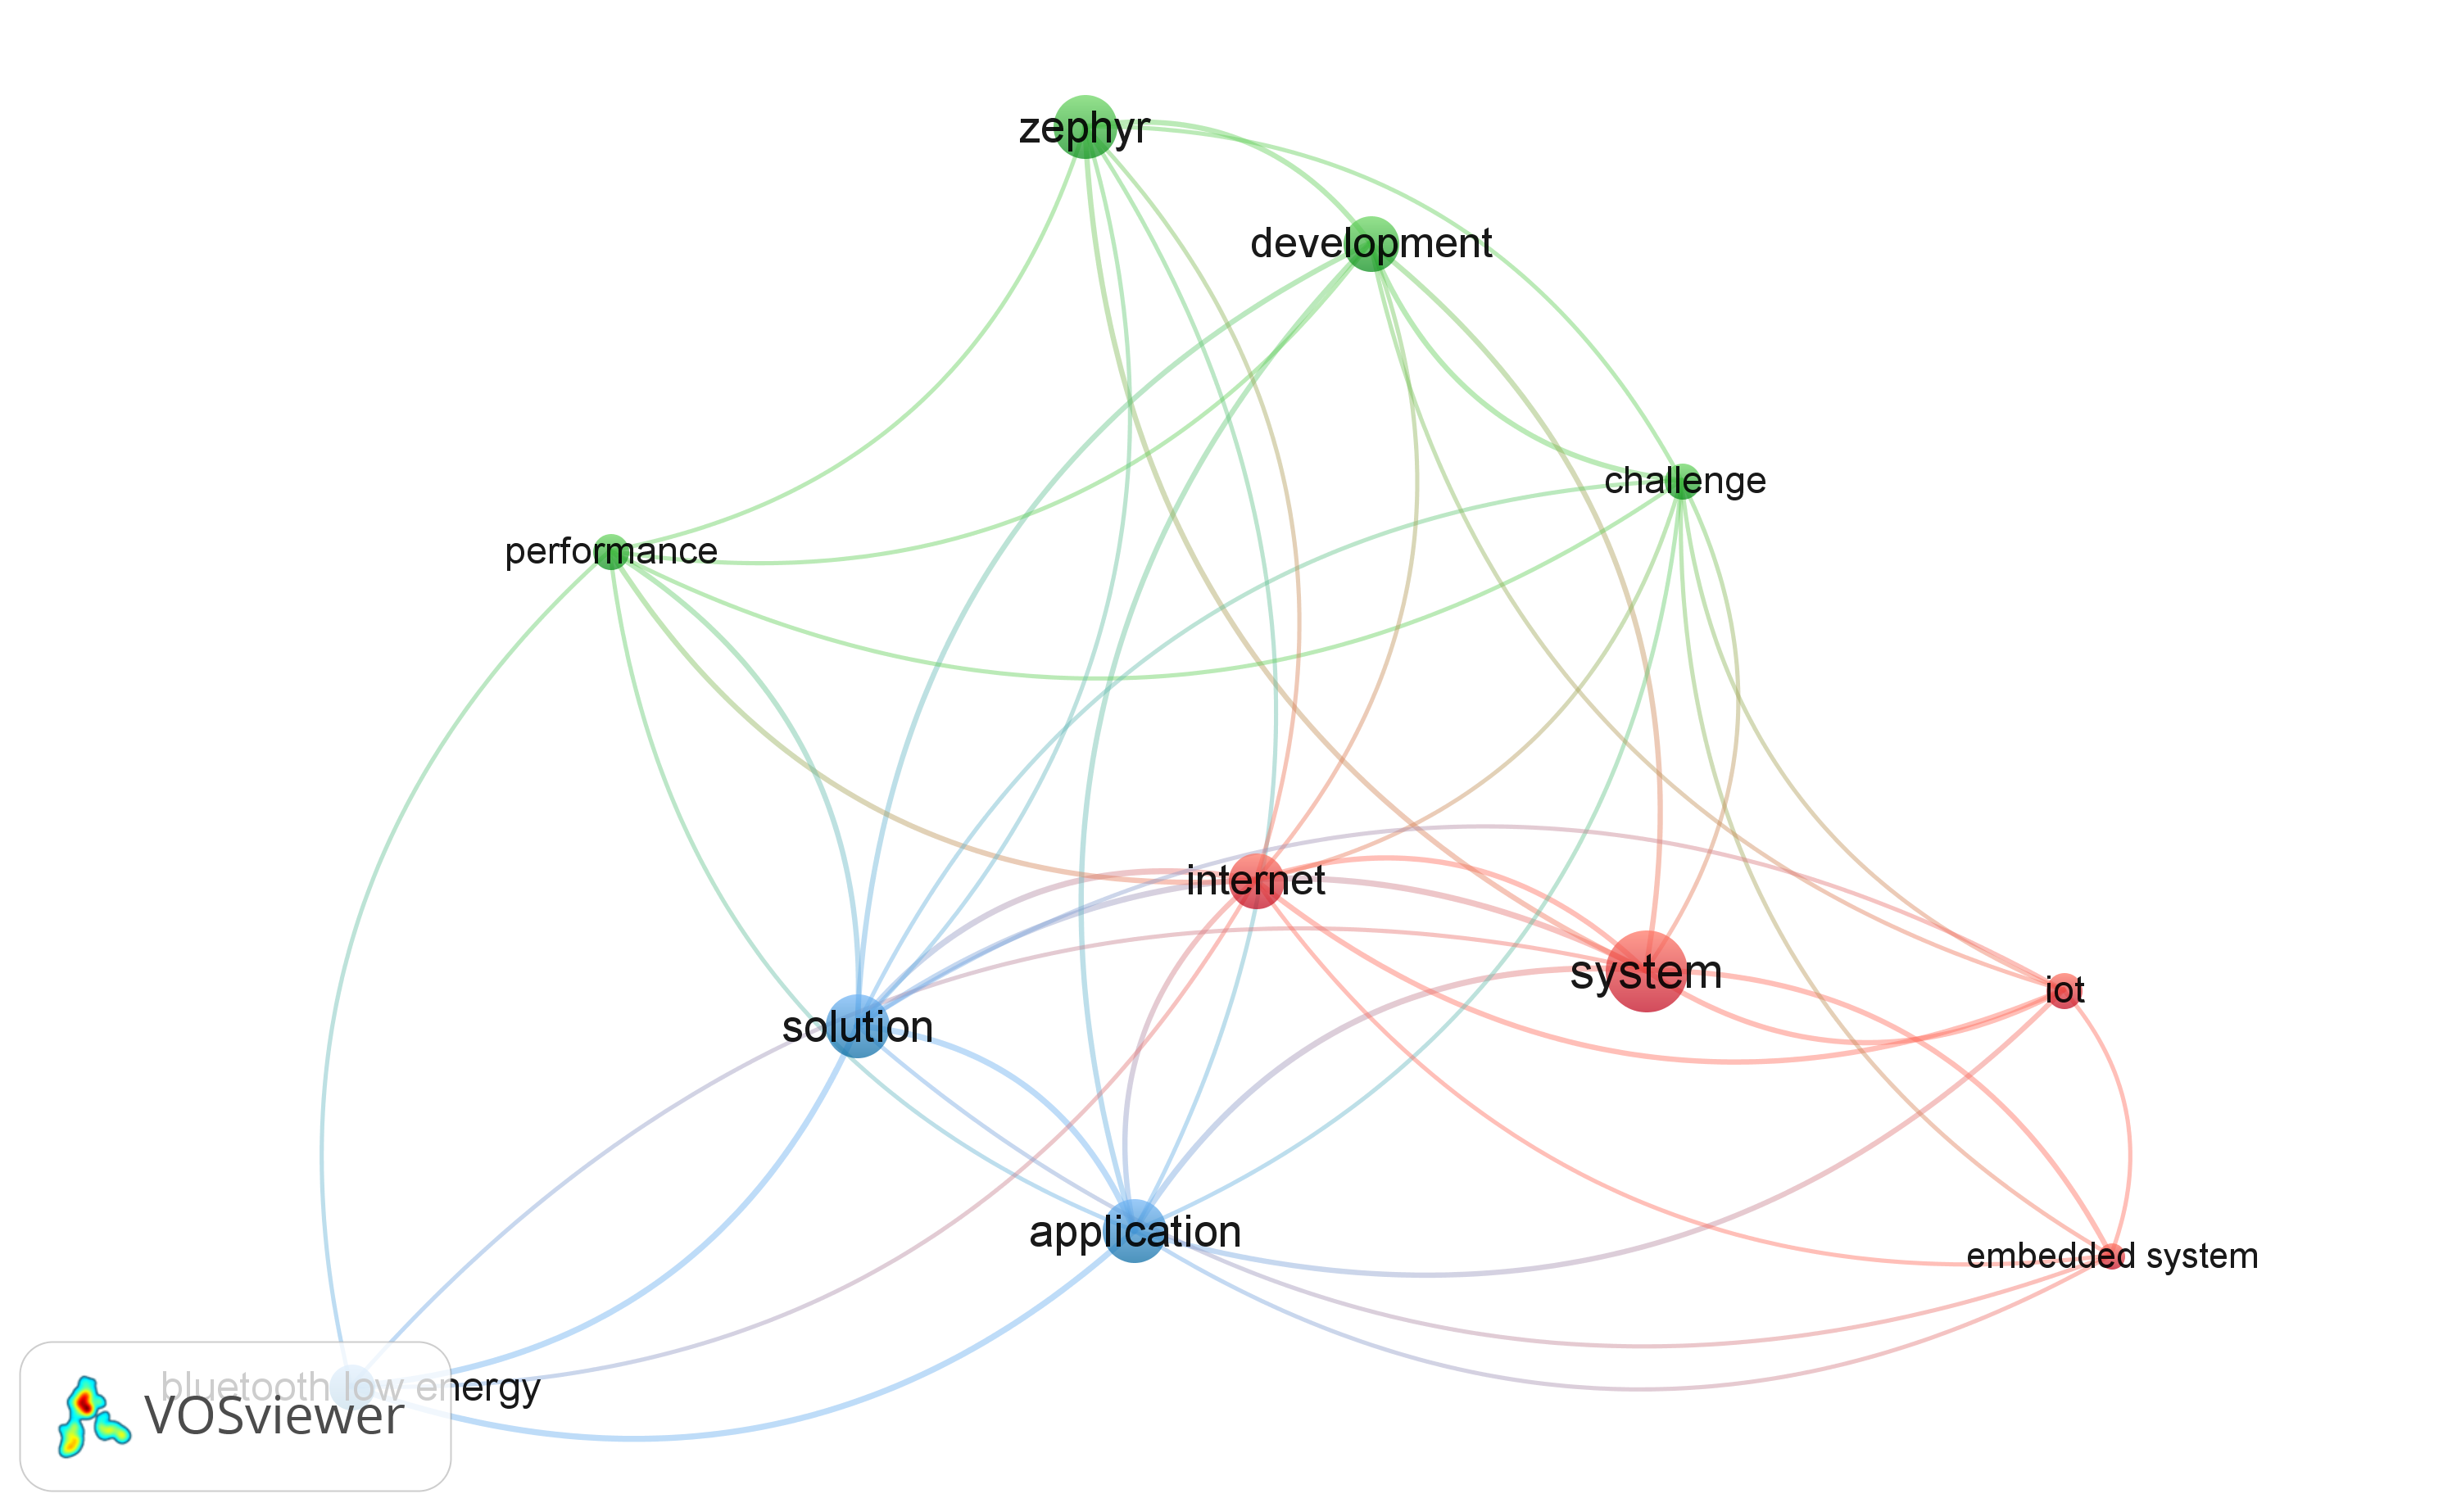
\includegraphics[width=15cm]{imagens/Zephyr_RTOS_Network_visualization.png}
	\caption{Mapa de visualização de rede sobre o termo "Zephyr RTOS"}
	Fonte: Autor com base no Software VOSViwer.
	\label{fig: Zephyr Network Visualization}
\end{figure}

A Figura~\ref{fig: Zephyr Network Visualization} demonstra uma rede de conexões entre o termo "Zephyr RTOS" 
e outros termos populares em sua pesquisa, nota-se conexões importantes entre zephyr e termos importante sem 
sua área. O tempo iot esta diretamente ligado a sistemas embarcados, sendo ligado ao zephyr através do termo 
"internet", o sistema é construído e mantido por diferentes empresas que trabalham no campo IOT 
\cite{huber_porting_2019}.


\subsection{Software CubeSat}
Para afunilar este estudo bibliométrico mais especifico para o termo central deste trabalho, realizou-se o 
levantamento sobre os termos "Cubesat SO", na base de trabalhos e citações Google Acadêmico, foi selecionado 
do período de 2012 a 2021 sendo encontrados aproximadamente 16.900 resultados, entre artigos, livros, 
citações e outros materiais acadêmicos. CubeSats são pequenos satélites limitados a cubos de 10cm³ atualmente 
muito populares, criado por Dr. Jordi Puig-Suari e Bob Twiggs, sendo uma espaçonave de custo e lançamento 
relativamente acessível \cite{Manyak2011FaultTA}. Na Figura~\ref{fig: Cubesat Density Visualization}nota-se 
os termos com mais destaques encontrados na busca feita neste trabalho.


\begin{figure}[H]
	\centering
	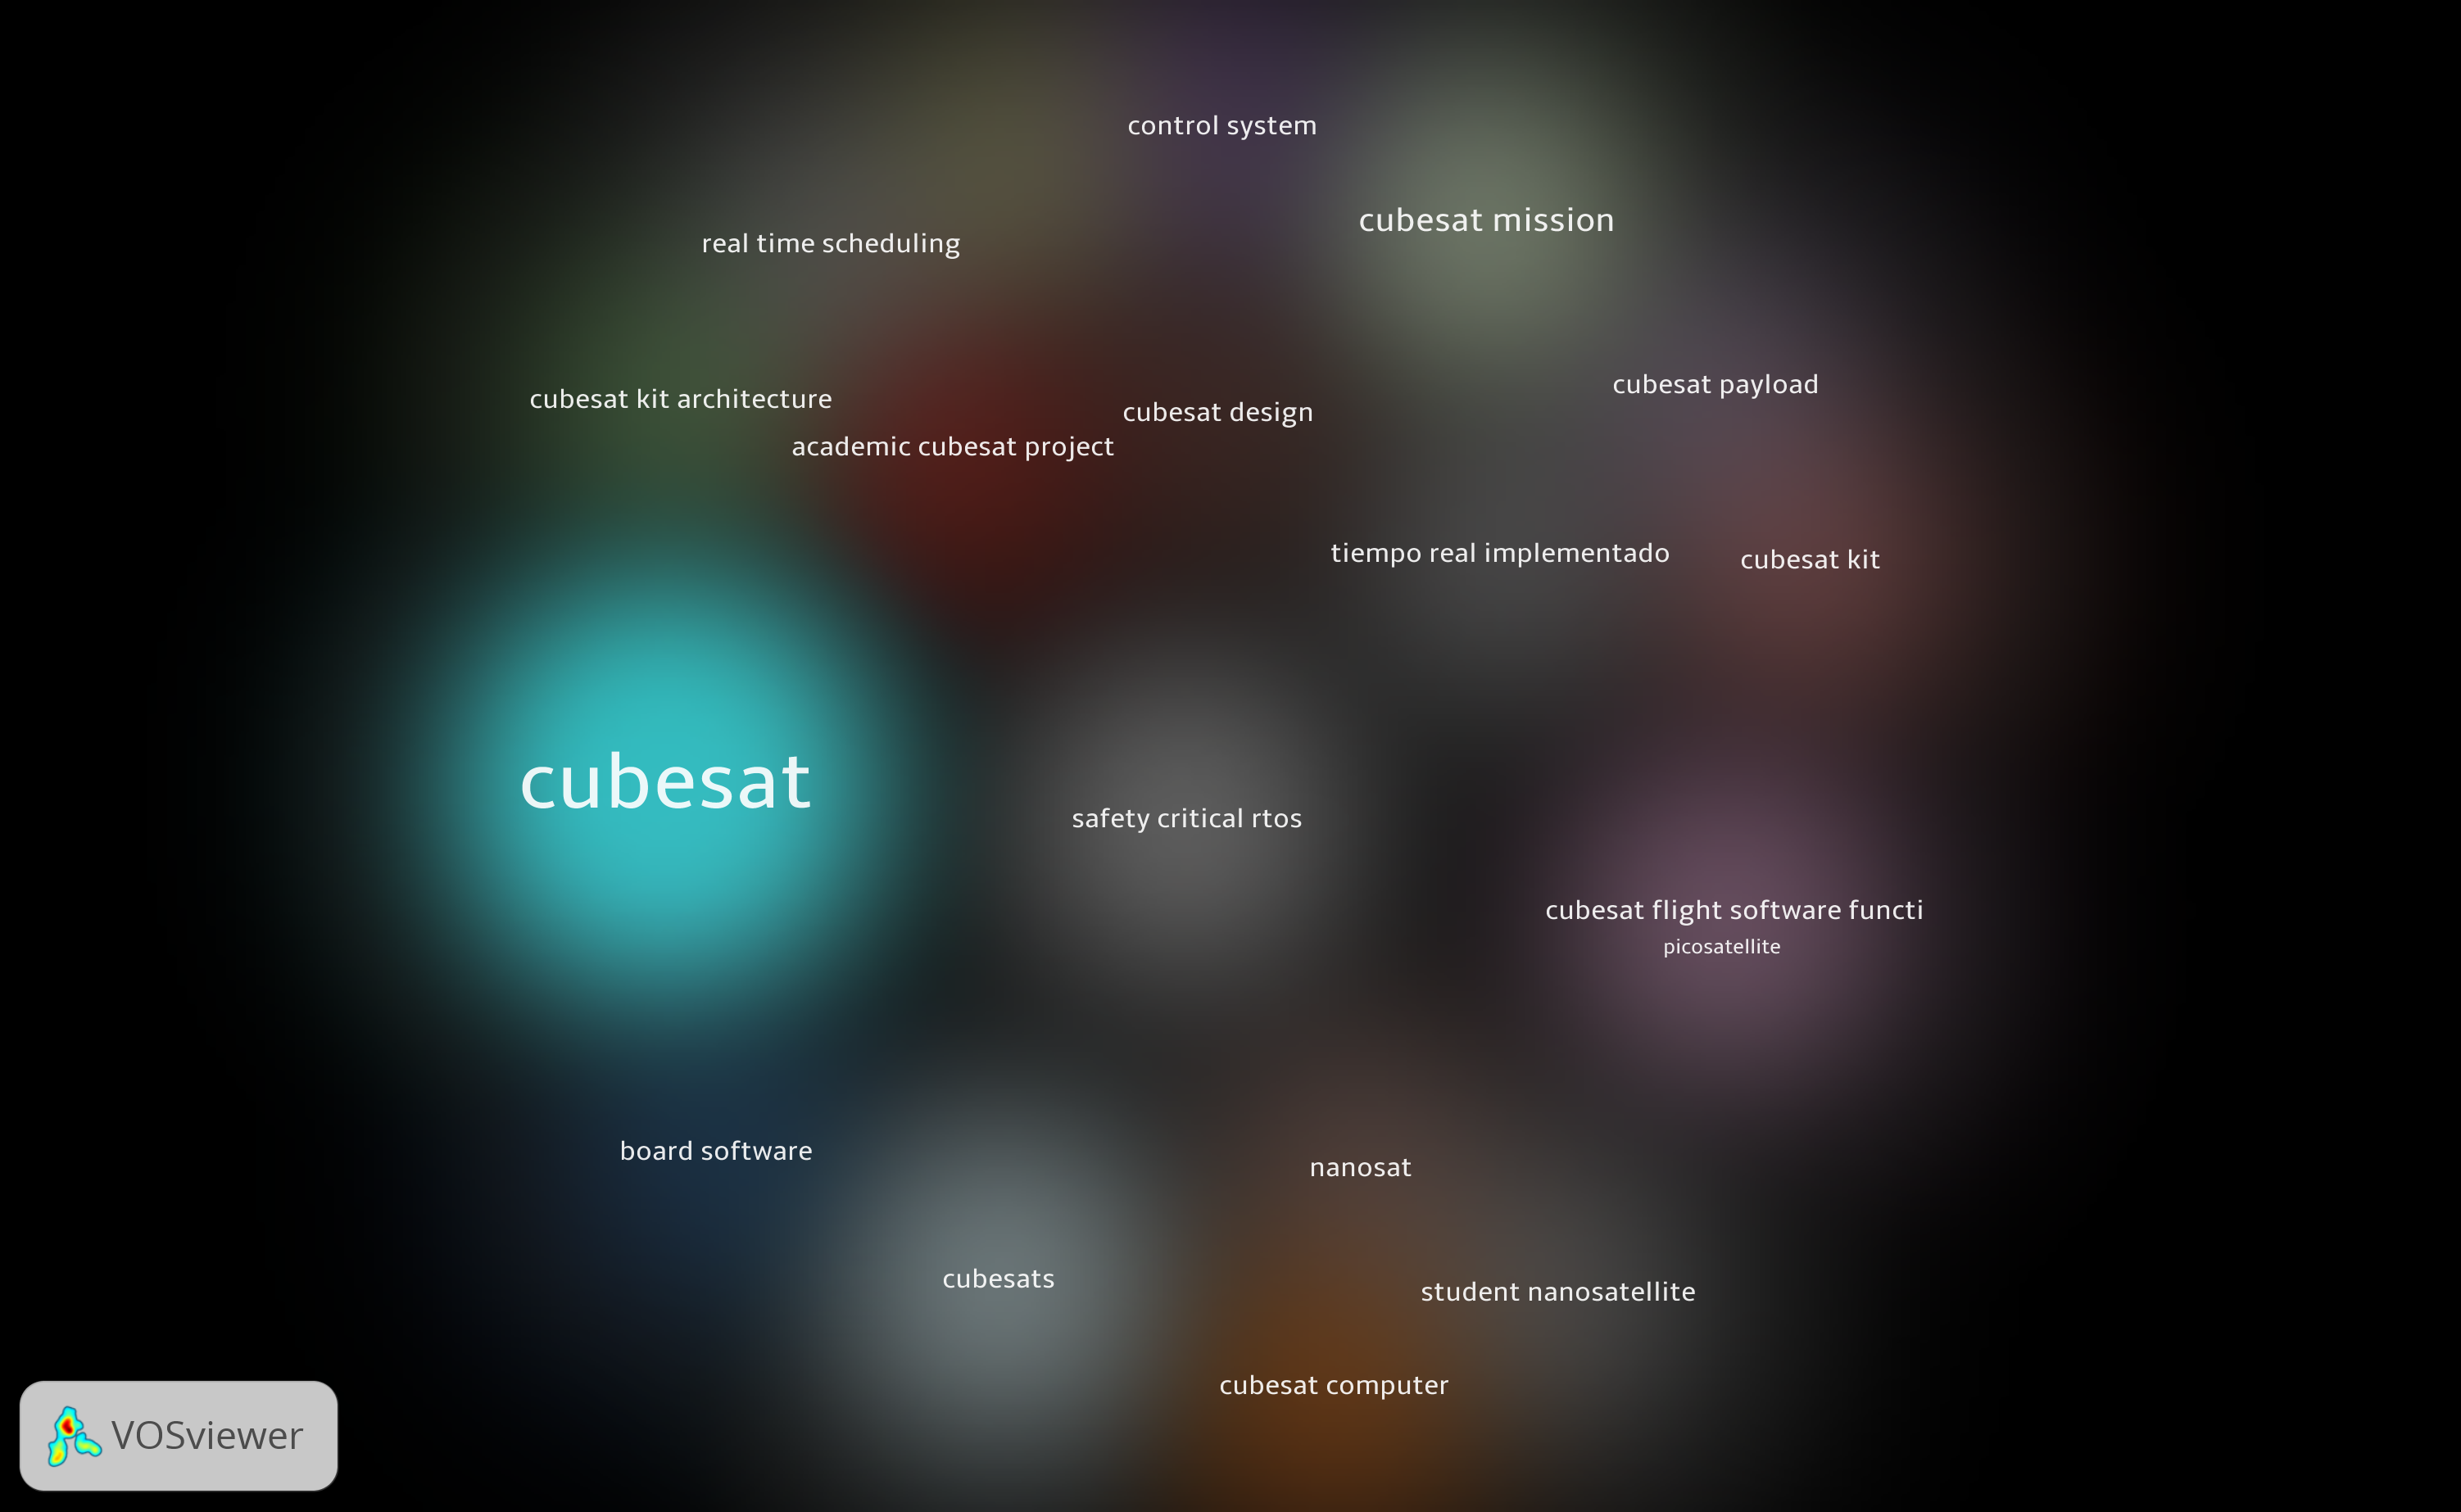
\includegraphics[width=15cm]{imagens/Cubesat_density_central.png}
	\caption{Mapa de visualização de densidade sobre o termo "Cubesat SO"}
	Fonte: Autor com base no Software VOSViwer.
	\label{fig: Cubesat Density Visualization}
\end{figure}

Ao redor do termo "cubesat", pode-se observar os termos correlacionado "academic cubesat project", 
"board software", "safety critical RTOS" e "cubesat kit architeture".Os cluster maiores e com cores mais 
vivas sinalizam um maior número de citações, a proximidade entre os termos indica correlação entre eles, 
todos os termos são encontrado sem trabalhos sobre cubesats, uma pesquisa na base de trabalhos Google 
Acadêmico retornou aproximadamente 16.900 resultados entre os anos de 2012 até 2021. Nota-se, na 
Figura~\ref{fig: Cubesat Published}, o número de trabalhos publicados por ano tem crescido a elevadas 
taxas anuais, chegando em 2020 com mais de 2.000 trabalhos publicados e citações contendo os termos 
"Cubesat SO" em título e resumo.


\begin{figure}[H]
	\centering
	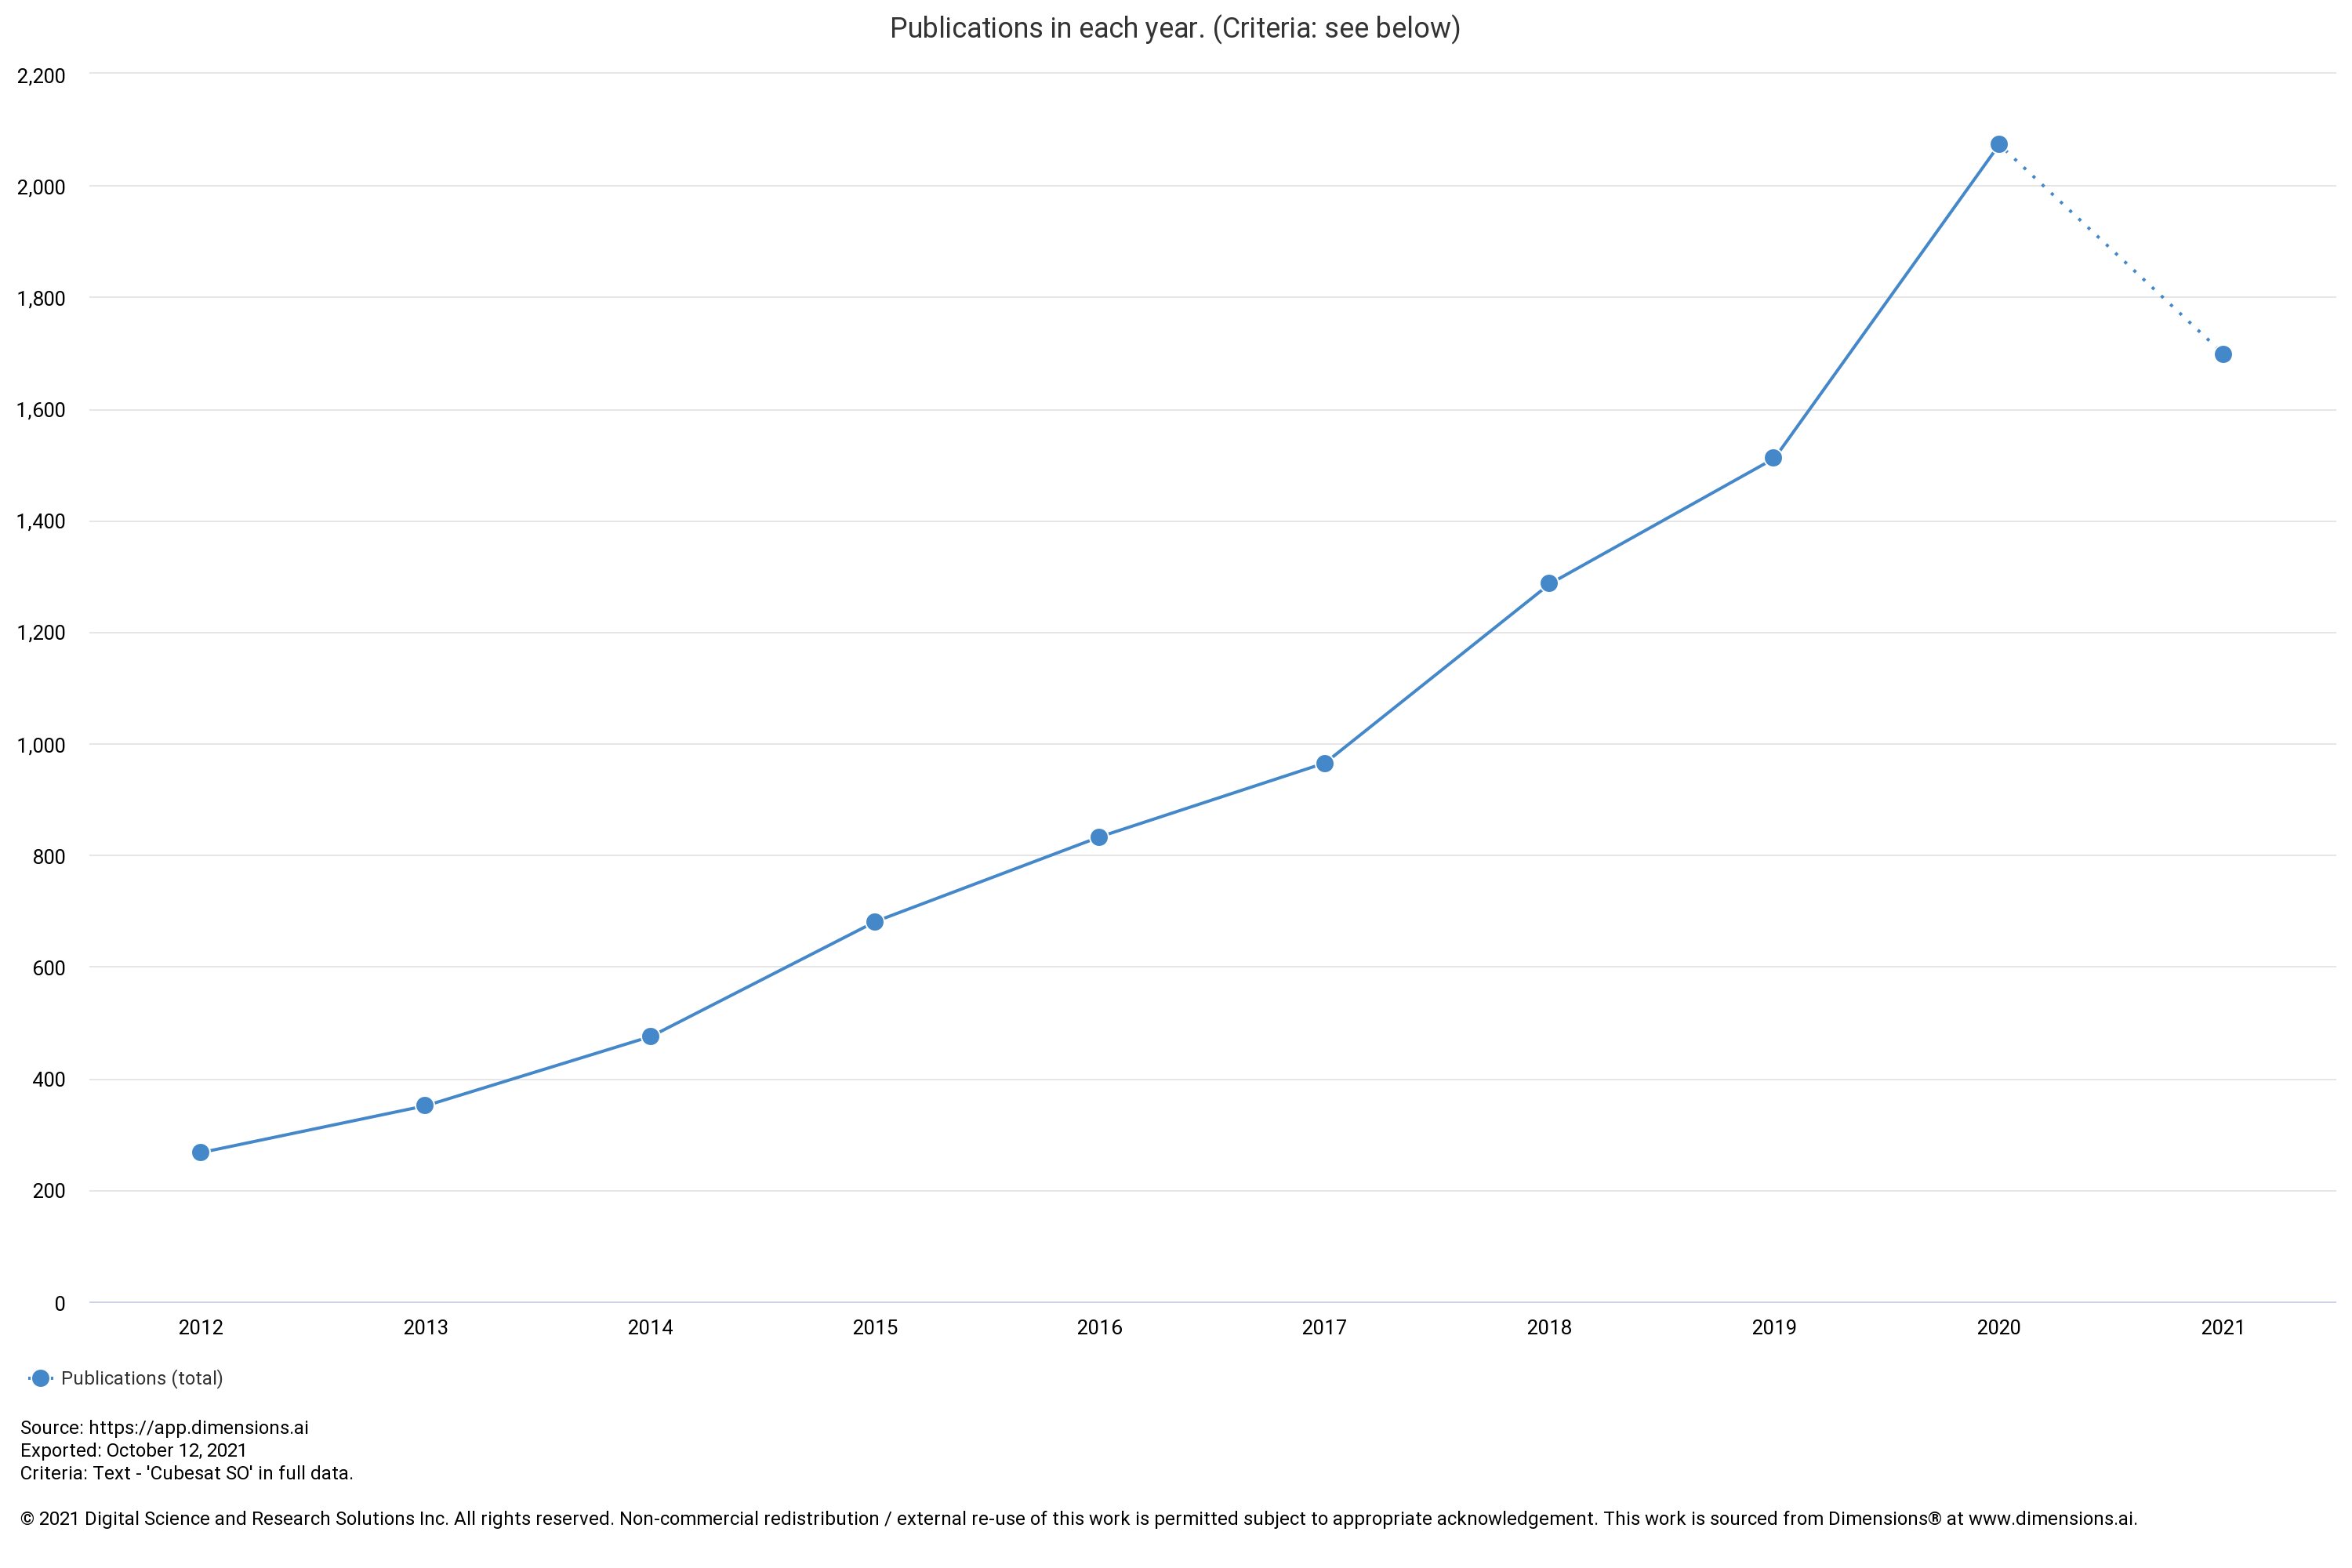
\includegraphics[width=15cm]{imagens/cubesat_publicados.png}
	\caption{A visualização mostra o número de publicações publicadas em cada ano de 2012 a 2021.}
	Fonte: Autor com base no site "dimensions.ai".
	\label{fig: Cubesat Published}
\end{figure}

Nota-se que o numero de trabalhos publicados e sempre maior que o ano anterior, reforçando a ideia de 
que os termos se encontram em destaque no meio acadêmico, com diversos trabalhos sendo correlacionados 
a iniciativas e nano satélites já concluídos ou em fase final de desenvolvimento. De acordo com \cite{Woellert2011} 
muitos destes projetos iniciam como spin-offs acadêmicos que terminam como uma atividade comercial.


\subsection{Conclusões sobre a Revisão Bibliométrica realizada}
% RTOS em CubeSats
Pode-se verificar a ocorrência de termos correlacionados nas duas pesquisas, com ênfase em 
"safety critical system" passando a ideia de conexão entre ambos, e interessante notar como 
os trabalhos sobre o projeto Zephyr tenta responder alguns dos problemas encontrados no 
desenvolvimento de um CubeSat, nota-se que o termo CubeSat e mais maduro do que o termo 
Zephyr, não encontrando nenhum trabalho relacionando os dois como um diferencial. 

% Ademais, 
% o levantamento bibliométrico passa a ideia que utilizar Zephyr em um projeto de Cubesat não 
% e uma ideia muito distante, abrindo uma janela de possíveis trabalhos na área que possam 
% trazer grandes contribuições, possibilitando o surgimento deste trabalho.

% Conclusão
